\documentclass[
  a4paper,
  11pt,
]{memoir}

%%~~~~~~~~~~~~~~~~~~~~~~~~~~~~~~~~~~~~~~~~~~~~~~~~~~~~~~~~~~~~
%% Layout

%% For temporary redefining the geometry of titlepage, bibliography, and
%% backcover.  Have to include here, otherwise it resets the Memoir layout.
\usepackage{geometry}

%% Stock size is same as page (A4).
\settrims{0pt}{0pt}

%% Line length set in Charter for 65 chars is ~26.5pc.  We go as low as possible
%% to give room to the margins.  Height is as large as possible (we don't use
%% the footer).
\settypeblocksize{627pt}{26pc}{*}

%% 2cm spine is enough (we need space here!).
\setlrmargins{2cm}{*}{*}

%% Don't have an opinion on header yet.  Just not too near to body text.
%% \setheadfoot{\baselineskip}{0pt}
\setheaderspaces{*}{4pc}{*}

%% Yeah margin notes!
\setmarginnotes{2pc}{15pc}{1pc}

\checkandfixthelayout

%%~~~~~~~~~~~~~~~~~~~~~~~~~~~~~~~~~~~~~~~~~~~~~~~~~~~~~~~~~~~~
%% General typography

%% TTF fonts with XeLaTeX.
\usepackage{fontspec}

%% Charter is an amazing body font.
\setromanfont{Charter}

%% Fira Sans is nice for the titles.
\setsansfont[
  BoldFont=FiraSans-Medium,
  ItalicFont=FiraSans-BookItalic,
  BoldItalicFont=FiraSans-MediumItalic,
  Scale=MatchUppercase
]{Fira Sans Book}

%% A monospace font that handles utf8 chars.  And is not too wide.
%% Scaled to match the body font.
\setmonofont[Scale=MatchUppercase]{Source Code Pro}

%% French typographical conventions and translated names for “Chapitre”, “Table
%% des matières”, etc.
\usepackage[french]{babel}

%% Move characters around and minimize hyphenation.  Good for diversity.  Not as
%% powerful with XeLaTeX, as font information may be missing.
\usepackage{microtype}

%% A touch of color
\usepackage{xcolor}
\definecolor{rubric}{rgb}{0.65,0.12,0.09}
\definecolor{azure}{rgb}{0.06,0.3,0.5}

%% Diagram colors
\definecolor{c0}{HTML}{556270}
\definecolor{c1}{HTML}{4ECDC4}
\definecolor{c2}{HTML}{FF6B6B}
\definecolor{c3}{HTML}{C7F464}

%%~~~~~~~~~~~~~~~~~~~~~~~~~~~~~~~~~~~~~~~~~~~~~~~~~~~~~~~~~~~~
%% Covers

%% Background image for first cover:
%% Paysage d'automne et d'hiver, Sesshū (end of 15th century)
\usepackage{eso-pic}
\newcommand\BackgroundPic{%
\put(0,0){%
\parbox[b][\paperheight]{\paperwidth}{%
\vfill
\centering
{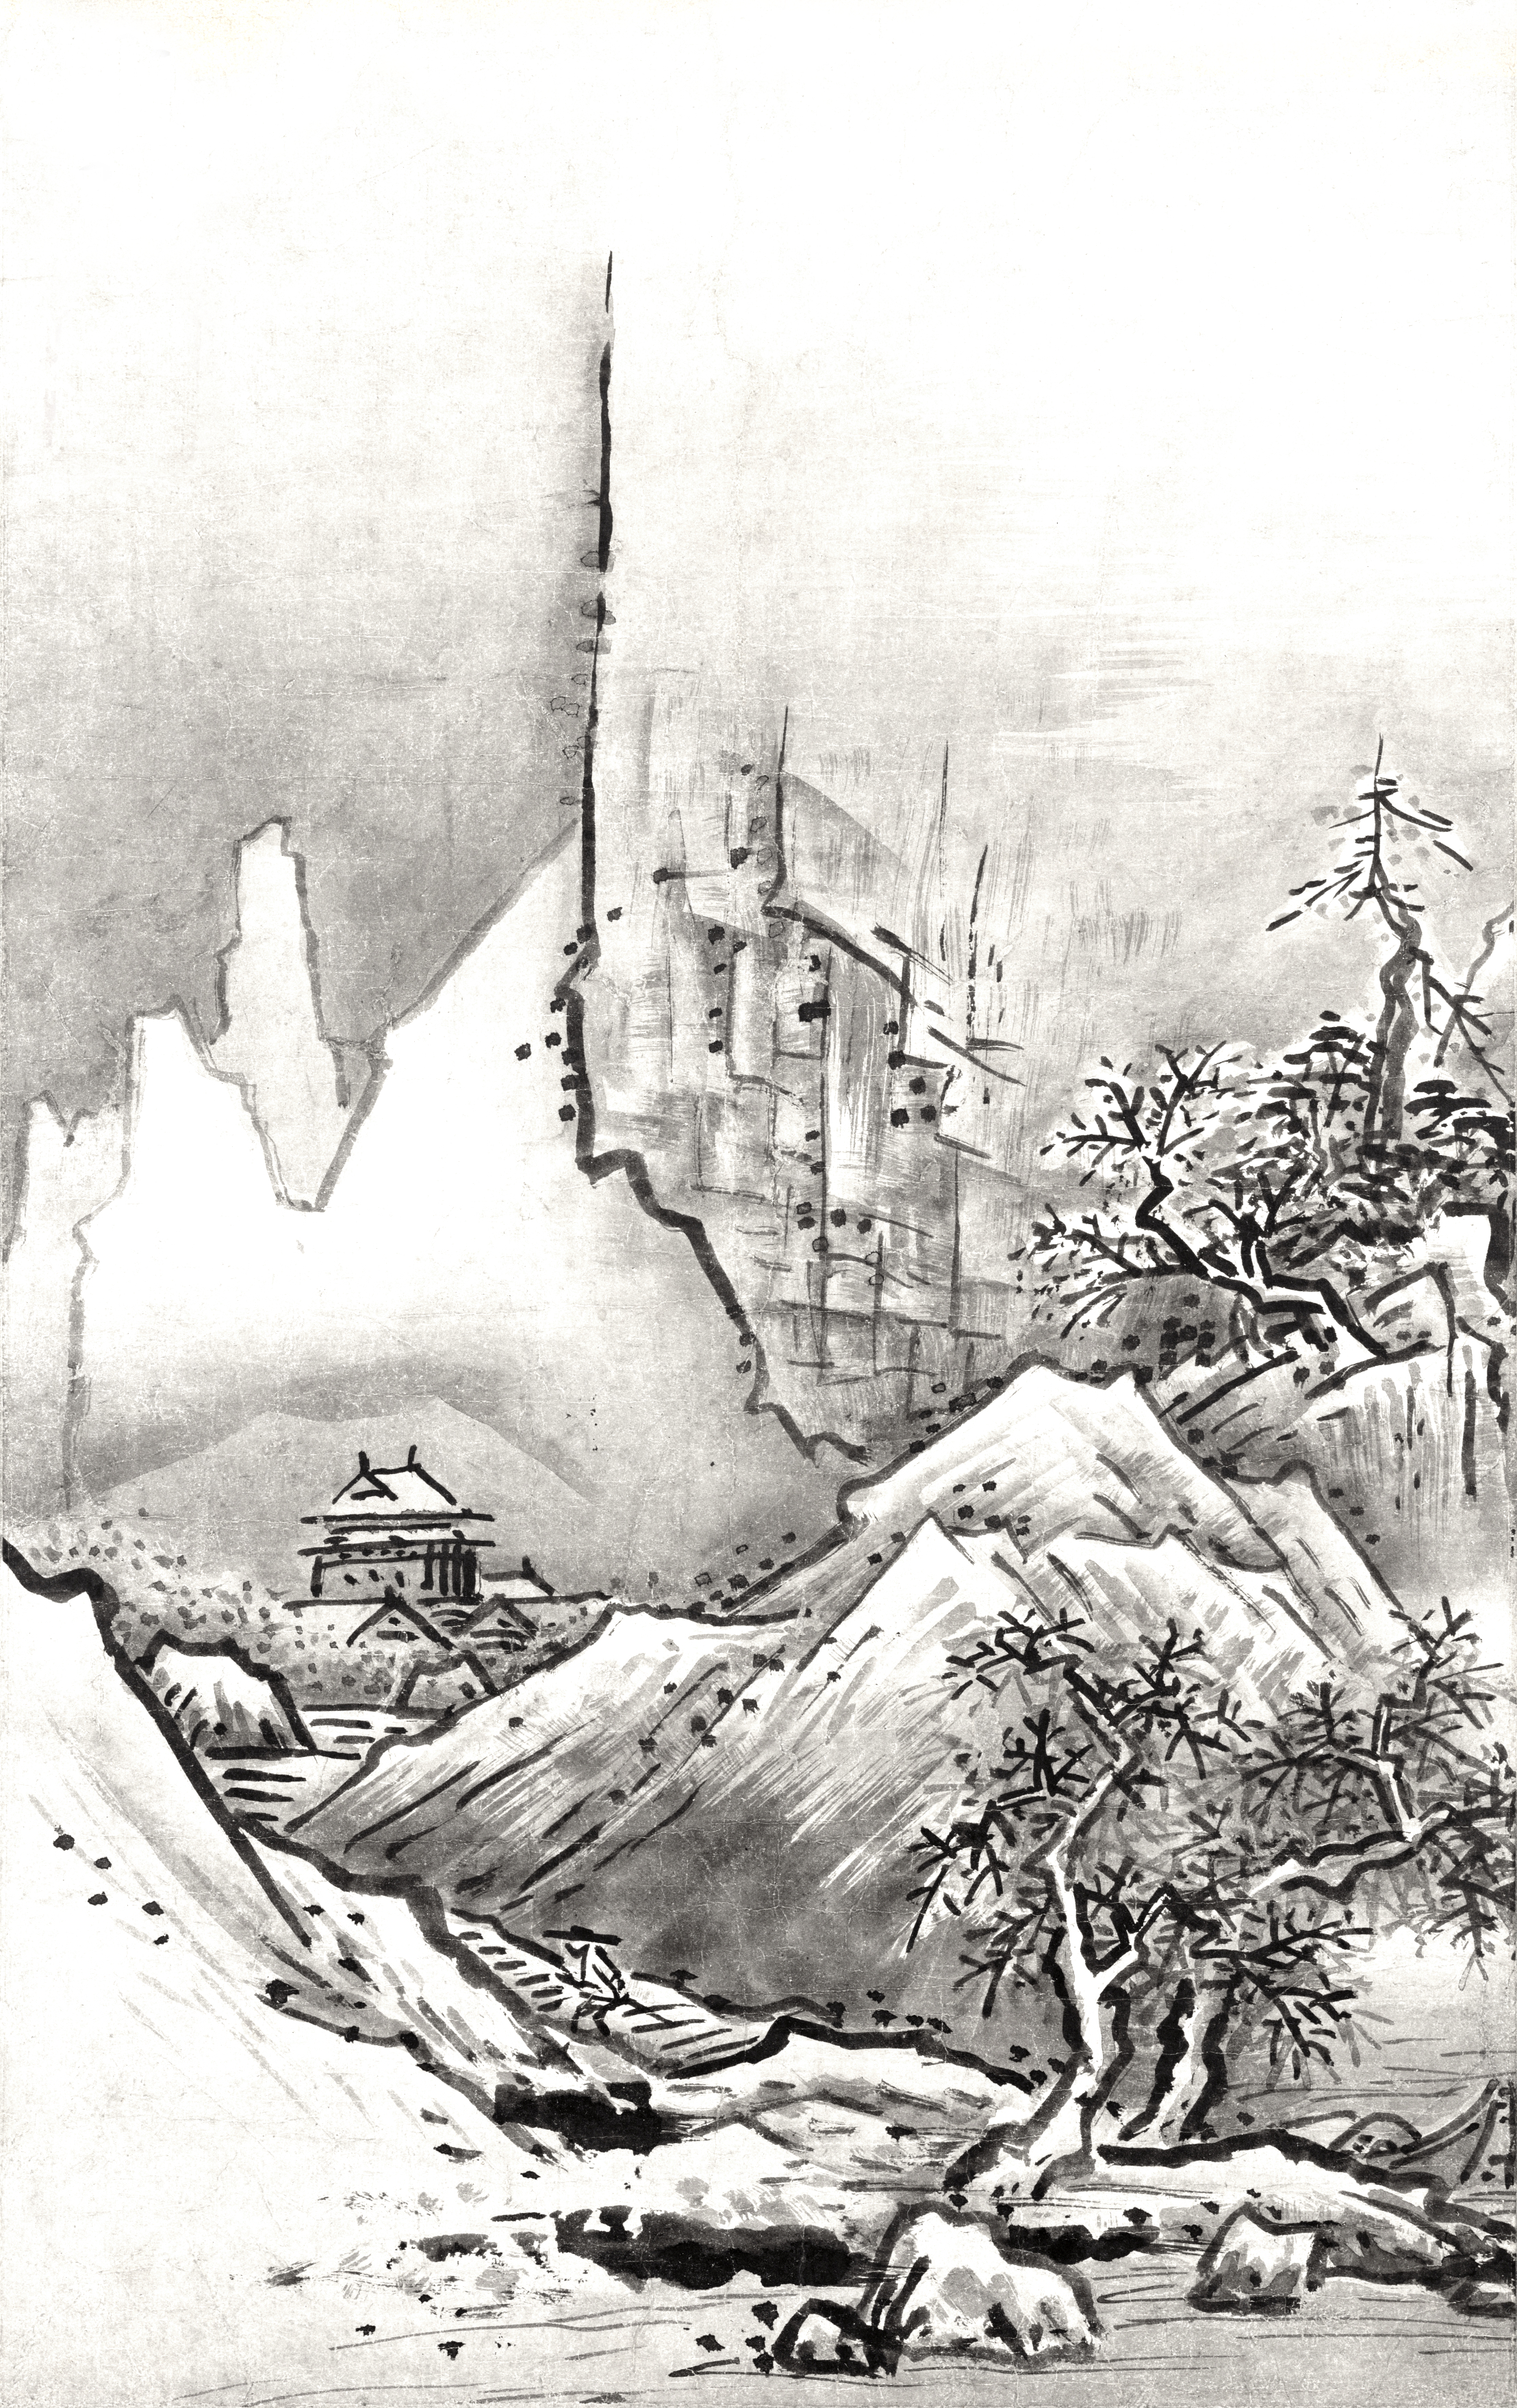
\includegraphics[width=\paperwidth,height=\paperheight,%
]{img/sesshu_sepia.jpg}}%
\vfill
}}}

%%~~~~~~~~~~~~~~~~~~~~~~~~~~~~~~~~~~~~~~~~~~~~~~~~~~~~~~~~~~~~
%% Headings

%% Sans-serif headings
\headstyles{komalike}

%% In-your-face chapter style
\chapterstyle{pedersen}
\renewcommand{\chaptitlefont}{\Huge\sffamily}
\renewcommand{\chapnumfont}{\sffamily\itshape}

%% Headers run into the margin
\setlength{\headwidth}{\textwidth}
\addtolength{\headwidth}{\marginparsep}
\addtolength{\headwidth}{\marginparwidth}
\makerunningwidth{headings}{\headwidth}
\makeheadposition{headings}{flushright}{flushleft}{}{}

%%~~~~~~~~~~~~~~~~~~~~~~~~~~~~~~~~~~~~~~~~~~~~~~~~~~~~~~~~~~~~
%% Side notes (in the outer margin)

%% For hyphenation in ragged text, which gives more even side notes.
\usepackage{ragged2e}

%% Marginpar is touchy to align vertically.  Marginnote is easier.
\usepackage{marginnote}
\renewcommand*{\raggedleftmarginnote}{\RaggedLeft}
\renewcommand*{\raggedrightmarginnote}{\RaggedRight}
\renewcommand*{\marginfont}{\small}

%% To refer to the body text of an environment using \BODY.
\usepackage{environ}

%% Aside is for side commentary.  Like footnotes, but in the margin.
\NewEnviron{aside}[1][0pt]{\marginnote{\BODY}[#1]}

%% Side figures are an image and a caption, both in the margin.
\NewEnviron{side-figure}[1][0pt]{\marginnote{\BODY}[#1]}

%% Babel french puts it in small caps.  I don’t want that.
%% Additionally, override figurename for listings.
%% HACK: maybe using a new environment for the listings would be a better
%% solution.
%% \newcommand{\UnsetListingFigureName}{\renewcaptionname{french}{\figurename}{Figure}}
%% \UnsetListingFigureName
%% \newcommand{\SetListingFigureName}{\renewcaptionname{french}{\figurename}{Code}}

%%~~~~~~~~~~~~~~~~~~~~~~~~~~~~~~~~~~~~~~~~~~~~~~~~~~~~~~~~~~~~
%% Epigraphs

\NewEnviron{epig}{\epigraph{\BODY}{}}
\setlength{\epigraphwidth}{20pc}
\setlength{\epigraphrule}{0pt}

%%~~~~~~~~~~~~~~~~~~~~~~~~~~~~~~~~~~~~~~~~~~~~~~~~~~~~~~~~~~~~
%% Source code listings

%% Environment for source code snippets.
\usepackage{listings}
\lstset{
  basicstyle=\ttfamily\small,
  commentstyle=\ttfamily\color{rubric},
  keywordstyle=,
  columns=fullflexible, keepspaces=true,
  breaklines=false, showstringspaces=false,
  escapeinside={//*}{\^^M},     % Escape to LaTeX between //* and line return
  %% aboveskip=-4pt,               % No space above and below, symmetric
  %% belowskip=0pt,
  %extendedchars=true, inputencoding=utf8,
}

%% Org export produces environment for ‘js’, so we must define that language for
%% listings.
\lstdefinelanguage{js}{
  language={Java},
  morekeywords={with,var,function},
  deletekeywords={double},
}

%% Accept the following’ as languages, no special treatment.  Otherwise listings
%% refuses to compile.
\lstdefinelanguage{diff}{}
\lstdefinelanguage{smalltalk}{}
\lstdefinelanguage{rust}{}
\lstdefinelanguage{elisp}{}
\lstdefinelanguage{asm}{}
\lstdefinelanguage{fortran}{}
\lstdefinelanguage{none}{}

%%~~~~~~~~~~~~~~~~~~~~~~~~~~~~~~~~~~~~~~~~~~~~~~~~~~~~~~~~~~~~
%% Bibliography

%% Quells a warning from biblatex with babel activated.  Not sure /what/ it does
%% though.
\usepackage{csquotes}

%% Generates the bibliography.  Handles UTF8-encoded bib files.
\usepackage[
  backend=biber,
  firstinits=false,
  sorting=nyt,                  % Sort by name, year, title
  backref=true,
  style=alphabetic,
  maxbibnames=10
]{biblatex}
\addbibresource{refs.bib}

%%~~~~~~~~~~~~~~~~~~~~~~~~~~~~~~~~~~~~~~~~~~~~~~~~~~~~~~~~~~~~
%% Others

%% Needed for the \text command in math-mode.
\usepackage{amsmath}

%% For including SVG (that are converted as PDF), and the JPEG illustrations.
\usepackage{graphicx}
%% This allows us to use width=\maxwidth{len} in \includegraphics to emulate the
%% CSS property max-width used by the HTML output.
%% Thanks: https://tex.stackexchange.com/questions/86350/includegraphics-maximum-width#86355
\makeatletter
\def\maxwidth#1{\ifdim\Gin@nat@width>#1 #1\else\Gin@nat@width\fi}
\makeatother

%% For color legend in diagrams
\newcommand{\colorrule}[1]{\textcolor{#1}{\rule{8pt}{4pt}}}

%% Hyperlinks for citations and external links.
\usepackage{hyperref}
\hypersetup{
  unicode,                      % Always a good idea?
  colorlinks=true,              % Color links rather than put boxes around them
  linkcolor=rubric,             % internal link
  citecolor=rubric,             % bibliography link
  urlcolor=azure,               % external link
}

%% Temporary handling of special blocks.
\newenvironment{full-figure}{}{}

%% Drop any FIXME.  The PDF is for reading!
\NewEnviron{fixme}{}


\newcommand{\titlefr}{Étendre des interpréteurs avec des mécanismes de langage}
\newcommand{\titleen}{Extending interpreters with language mechanisms}

\title{\titlefr}
\author{fmdkdd}

\begin{document}

%% Insert title, TOC, and acknowledgments.  The Org document must not insert
%% title or TOC itself, otherwise they will appear before the frontmatter
%% command.

\frontmatter

\begin{titlepage}
\sffamily
\vspace{6cm}

\begin{raggedright}
\Huge\titlefr
\end{raggedright}

\vspace{1.5cm}

\LARGE
\noindent
Florent \textsc{Marchand de Kerchove}

\vfill

%% To change the margins on this page (from KOMA):
%% \begin{addmargin}[0cm]{-4cm}
%% \end{addmargin}
\begin{raggedright}
\rmfamily\normalsize
\itshape
Thèse de doctorat présentée en vue de l'obtention du
grade de docteur de l'université de Nantes
sous le label de l'université de Nantes, Angers, Le Mans.

\vspace{1em}
École doctorale: sciences et technologies de l'information et mathématiques\\
Discipline: informatique, section CNU 27\\
Unité de recherche: laboratoire d'informatique de Nantes-Atlantique (LINA)\\

\vspace{1em}
Soutenue le 27 octobre 2016, devant le jury composé de:

\vspace{0.5em}
M. Hulu Berlu, professeur, Tartifrice, rapporteur;\\
M. Ali Barli, professeur, Hamilcar, examinateur;\\
M. Po Nan, professeur, Asifond, rapporteur;\\
M. Jacques Noyé, maître-assistant, Mines Nantes, encadrant de thèse;\\
M. Mario Südholt, professeur, Mines Nantes, directeur de thèse.\\
\vspace{-2cm}
\end{raggedright}
\end{titlepage}

\tableofcontents

%% \chapter*{Remerciements}
%% %% Fix heading mark showing “Contents”
%% %% as suggested here:
%% %% https://en.wikibooks.org/wiki/LaTeX/Document_Structure#The_document_environment
%% \markboth{\MakeUppercase{Remerciements}}{}
%% \input{acks}

\mainmatter
\input{manuscript}

%% Back matter for bibliography, eventual index.

\backmatter

\addcontentsline{toc}{part}{Bibliography}
\printbibliography
%% Back cover
\newcommand{\heading}[1]{{\sffamily\textbf{#1}\vspace{4pt}}}

\begin{titlepage}
\vspace{2cm}
\begin{addmargin}[-1cm]{-4cm}
\begin{flushright}
\sffamily\LARGE\titleen
\end{flushright}
\vfill
\noindent
\begin{minipage}[t]{9cm}

\heading{Résumé}\\
Nullam eu ante vel est convallis dignissim.  Fusce suscipit, wisi nec facilisis
facilisis, est dui fermentum leo, quis tempor ligula erat quis odio.  Nunc porta
vulputate tellus.  Nunc rutrum turpis sed pede.  Sed bibendum.  Aliquam posuere.
Nunc aliquet, augue nec adipiscing interdum, lacus tellus malesuada massa, quis
varius mi purus non odio.  Pellentesque condimentum, magna ut suscipit
hendrerit, ipsum augue ornare nulla, non luctus diam neque sit amet urna.
Curabitur vulputate vestibulum lorem.  Fusce sagittis, libero non molestie
mollis, magna orci ultrices dolor, at vulputate neque nulla lacinia eros.  Sed
id ligula quis est convallis tempor.  Curabitur lacinia pulvinar nibh.  Nam a
sapien.

Aliquam erat volutpat.  Nunc eleifend leo vitae magna.  In id erat non orci
commodo lobortis.  Proin neque massa, cursus ut, gravida ut, lobortis eget,
lacus.  Sed diam.  Praesent fermentum tempor tellus.  Nullam tempus.  Mauris ac
felis vel velit tristique imperdiet.  Donec at pede.  Etiam vel neque nec dui
dignissim bibendum.  Vivamus id enim.  Phasellus neque orci, porta a, aliquet
quis, semper a, massa.  Phasellus purus.  Pellentesque tristique imperdiet
tortor.  Nam euismod tellus id erat.

Nullam eu ante vel est convallis dignissim.  Fusce suscipit, wisi nec facilisis
facilisis, est dui fermentum leo, quis tempor ligula erat quis odio.  Nunc porta
vulputate tellus.  Nunc rutrum turpis sed pede.  Sed bibendum.  Aliquam posuere.
Nunc aliquet, augue nec adipiscing interdum, lacus tellus malesuada massa, quis
varius mi purus non odio.  Pellentesque condimentum, magna ut suscipit
hendrerit, ipsum augue ornare nulla, non luctus diam neque sit amet urna.
\end{minipage}%
\hspace{1cm}%
\begin{minipage}[t]{9cm}
\heading{Abstract}\\
Programs are hard to write, and harder to maintain.  Programs are often part of
an /ongoing/ development process: they evolve as requirements change, as new
features are added, and as defects are uncovered and fixed.  Following the
impulse of agile methodologies that prone rapid iteration, programs can be
considered from the start as being in this permanent state of maintenance.

Programmers need tools to ease the maintenance of programs.  New programming
languages are created every day to enhance the productivity of programmers, to
simplify the conception of programs.  Object-Oriented Programming,
Metaprogramming, Aspect-Oriented Programming, Feature-Oriented Programming,
Functional Programming: all promise a better way to write safer programs.  But
how do these paradigms help /maintain/ programs?

We
\end{minipage}

\vfill
\noindent
\begin{minipage}[t]{9cm}
\heading{Mots-clés}\\
Extensibilité, modularité, interpréteurs, instrumentation, patrons de
conception, programmation par objets, programmation par aspects, JavaScript,
langages de programmation.
\end{minipage}%
\hspace{1cm}
\begin{minipage}[t]{9cm}
\heading{Keywords}\\
Extensibility, modularity, interpreters, instrumentation, Design Patterns,
Object-Oriented Programming, Aspect-Oriented Programming, JavaScript,
programming languages.
\end{minipage}
\end{addmargin}
\end{titlepage}

\end{document}
